\section*{3.1b)}

Zu zeigen ist der Zusammenhang, der zwischen der logistischen Abbildung mit $r = 4$
\begin{equation}
 M_L(x_n) = 4x_n(1-x_n) = x_{n+1}
 \label{eqn:ml}
\end{equation}
und der Dreiecksabbildung
\begin{equation}
 \label{eqn:md}
 M_D(x_n) = \left(1-2\left|\frac{1}{2}-x\right|\right) = x_{n+1}
\end{equation}
besteht.

Nun substituieren wir $x_n$ in \eref{ml} mit:
\begin{equation}
 x_n = \sin^2\left(\frac{\pi}{2}\alpha_n\right)
\end{equation}
Hierbei wird darauf geachtet, dass die Substitution selbst auch eine Abbildung
von $[0, 1]$ nach $[0, 1]$ darstellt. Man erhält:
\begin{eqnarray}
 M_L(x_n) = x_{n+1} &=& 4x_n(1-x_n) \\
 \sin^2\left(\frac{\pi}{2}\alpha_{n+1}\right) &=& 4\sin^2\left(\frac{\pi}{2}\alpha_n\right)\underbrace{\left(1-\sin^2\left[\frac{\pi}{2}\alpha_n\right]\right)}_{\cos^2\left(\frac{\pi}{2}\alpha_n\right)} \\
 &=& 4\left[ \sin\left(\frac{\pi}{2}\alpha_n\right)\cos\left(\frac{\pi}{2}\alpha_n\right)\right]^2 = 4 \left[ \frac{1}{2} \sin\left( 2 \frac{\pi}{2} \alpha_n \right) \right]^2 = \sin^2\left(\frac{\pi}{2}2\alpha_n\right) \\
 \rightarrow \alpha_{n+1} &=& \pm 2 \alpha_n
\end{eqnarray}

Wie aus der Vorlesung bekannt ist, hat die logistische Abbildung ebenfalls eine
Stretching-Wirkung mit Faktor 2. Das Vorzeichen hängt hierbei von $x$ ab und ist
für Werte $\in [0; 0.5]$ positiv.

Darauf folgt die Equivalenz des invarianten Maßes der Dreiecksabbildung $ρ_D = 1$
und der logistischen Abbildung in Abhängigkeit von $alpha$ $ρ_L(α)$:
\begin{equation}
 ρ_D = ρ_L(α) = 1 
\end{equation}
Es gilt weiterhin:
\begin{eqnarray}
 ρ_L(α)\dd{α} &=& ρ_L(x)\dd{x} \\
  \rightarrow ρ_L(x) &=& \underbrace{ρ_L(α)}_{=1} \frac{\dd{\alpha}}{\dd{x}} \\
 \frac{\dd{x}}{\dd{α}} &=&  π \sin\left(\frac{\pi}{2}\alpha\right)\cos\left(\frac{\pi}{2}\alpha\right) = π\sqrt{x(1-x)} \\
 \rightarrow ρ_L(x) &=& \frac{1}{\pi\sqrt{x(1-x)}}
\end{eqnarray}

Der Vergleich zwischen experimentellem und theoretischem Ergebnis ist in \fref{1b}
veranschaulicht. Die rote Line beschreibt den auf die experimentellen Daten
renormierten theroretischen Verlauf $ρ_L(x)$.
\begin{figure}[htb]
\centering
  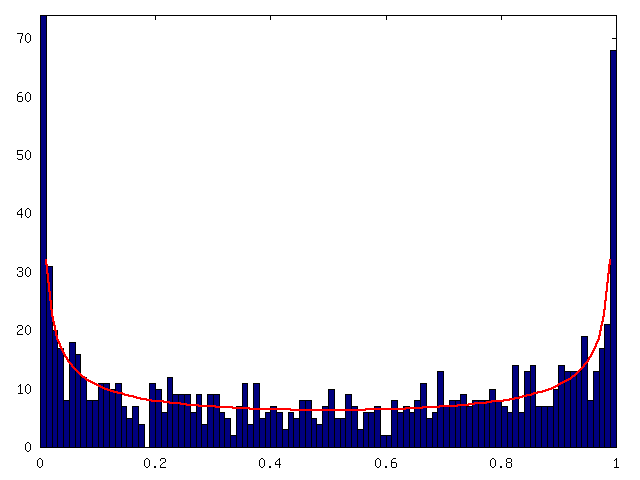
\includegraphics[width=1\columnwidth,keepaspectratio]{../logabb_r4.png}
  \caption{Vergleich zwischen Experiment und Theorie von $ρ_L(x)$}
  \label{fig:1b}
\end{figure}





